\section{Bonus 2: Anàlisi no supervisat de les dades}
% Fer an`alisi no supervisat de les dades. Traient la variable ”Status”, podem identificar cl ́usters? A què corresponen? Ens poden servir per quelcom en la nostra tasca? I fora de la nostra tasca?

En aquest apartat s'ha volgut realitzar un anàlisis no supervisat de les dades d'entrenament. Aquest estudi es farà sobre les dades d'entrenament utilitzades en el model escollit (amb les mateixes modificacions realitzades respecte la base de dades original, però eliminant la variable \textit{Status}).

Per realitzar aquest anàlisi no supervisat, s'ha volgut trobar clústers (grups) de mostres a dins de tot el conjunt. Generalment el clustering es pot fer amb algoritmes com k-means, hierarchical clustering, etc. En aquest cas, donat que no es coneix quin nombre de clústers hi ha en la base de dades, s'ha decidit realitzar un clustering jeràrquic (hierarchical clustering).

Per realitzar aquest clustering s'executarà la funció \texttt{hierarchical\_clustering()}. El mètode que s'ha escollit per calcular les distàncies entre individus de la base de dades és el linkage de \textit{Ward}, que intenta reduir al màxim la variància en cada un dels clústers. Per tal de poder calcular distàncies entre variables categòriques, es realitza un \textit{One Hot Encoding}.

Una vegada es troben els diferents clústers, s'ha fet un dendograma on es poden visualitzar fàciliment tots els clusters. El podem trobar en la figura \ref{fig:dendogram} i es pot veure que s'han detectat clarament 4 clusters.

\begin{figure}[H]
	\centering
	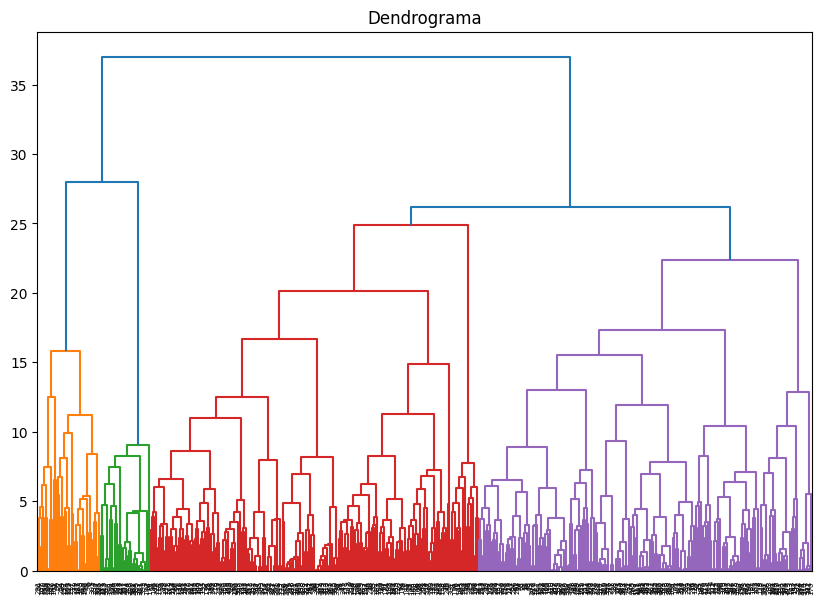
\includegraphics[width=0.85\linewidth]{img/dendogram.png}
	\caption{Dendograma amb els diferents clusters diferenciats.}
	\label{fig:dendogram}
\end{figure}

Els dos clústers de la dreta contenen clarament més dades que la resta, de manera que això pot portar problemes a la hora de fer un profiling (interpetació dels clusters).

Per visualitzar els clusters d'una altra manera, s'ha fet un ACPi s'han projectat les mostres en els dos primers components principals (que ens expliquen aproximadament un 35\% de la variància). En la figura \ref{fig:clust-acp} es pot veure com els clústers estan prou distingits entre ells, de manera que sembla que el hierarchial clustering s'ha realitzat correctament.

\begin{figure}[H]
	\centering
	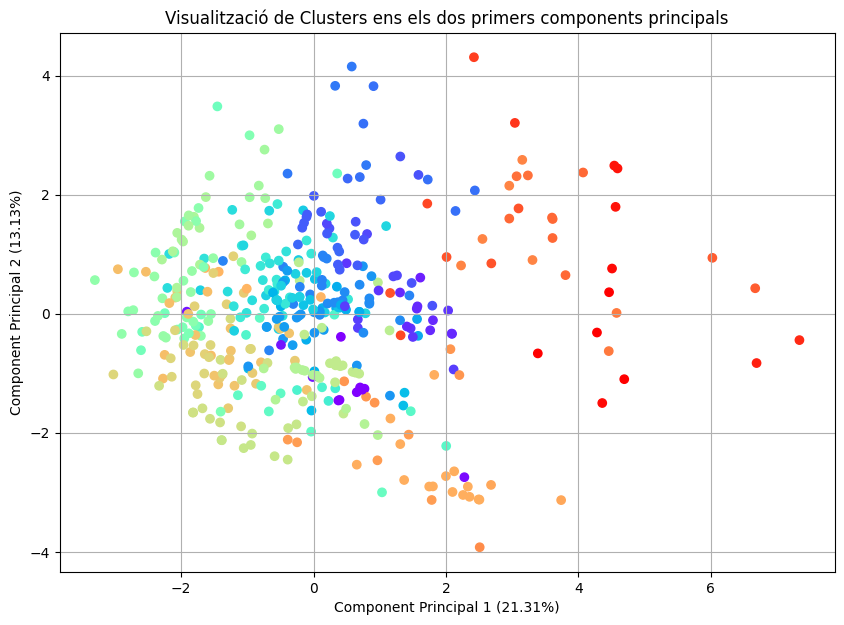
\includegraphics[width=0.85\linewidth]{img/clust-acp.png}
	\caption{Visualització dels diferents clusters en els dos primers components principals d'un ACP. Els colors dels clústers s'haurien de perfeccionar per millorar la interpretació.}
	\label{fig:clust-acp}
\end{figure}

A continuació s'hauria de realitzar el profiling dels diferents grups (clusters). Això es pot fer comparant les mitjanes i distribucions de les variables numèriques en cada un dels diferents clusters, així com comparant la proporció de cada classe de les variables categòriques en cada grup.

Amb tot això s'aconseguiria etiquetar cada un dels grups i es podria extreure molta informació sobre quins diferents tipus de pacients amb Cirrosi hi ha. Posteriorment, en relació al nostre estudi, es podria comparar la proporció de cada clúster respecte a la variable objectiu de tot l'estudi, per tal de determinar si els grups de pacients que s'han trobat tenen probabilitats diferents de sobreviure a la malaltia. El més esperable és que els grups estiguin separats per criteris semblants als que s'han vist anteriorment en aquest projecte en l'estudi de la dimensionalitat per els dos primers components principals.

Lamentablement, en aquest treball no ha donat temps de poder realitzar aquest profiling dels diferents clusters. No obstant, s'han pogut fer uns bons primers passos d'aquest anàlisis no supervisat de les dades que es podrien continuar, tal i com s'ha indicat, per arribar a més conclusions interessants.